\chapter{Cambios en la interfaz administrativa de ePhoenix}
\label{apendiceA}
\lhead{Apéndice A. \emph{Cambios en la interfaz administrativa de ePhoenix}}

% En los apéndices se incluye cualquier información que no sea esencial para la
% comprensión básica del trabajo, pero provea ejemplos y casos de estudio
% extendidos que permitan un análisis más exhaustivo.

\begin{figure}[h!]
\centering
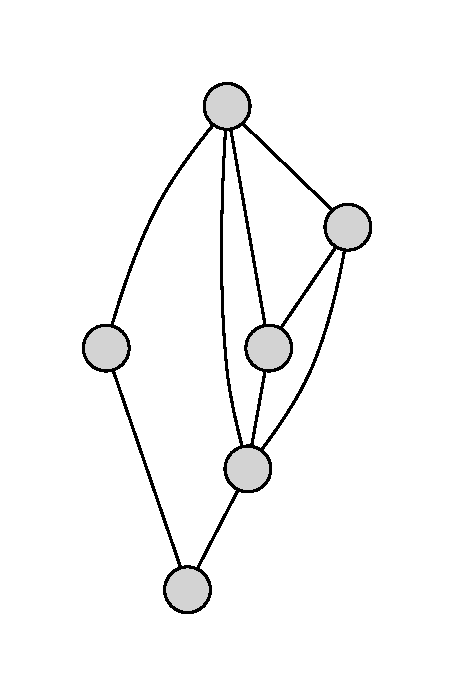
\includegraphics[width=0.5\textwidth]{grafo}
\caption[Grafo]{Grafo gris.}
\label{imagen:grafo}
\end{figure}

\begin{figure}[h!]
\centering
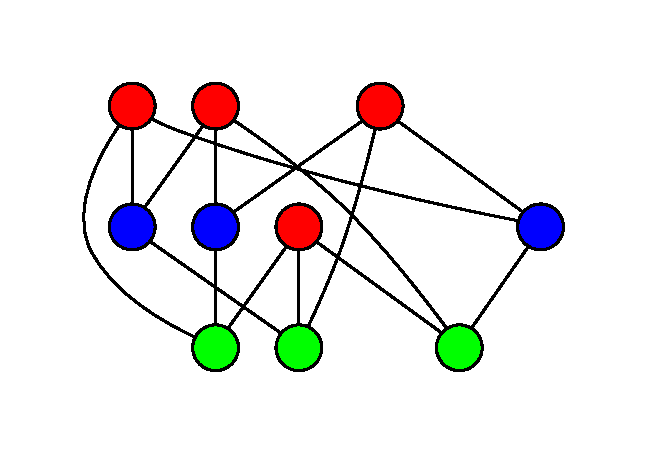
\includegraphics[width=\textwidth]{grafocolor}
\caption[Grafo coloreado (esto sale en la tabla de contenidos)]{Grafo con color.}
\label{imagen:grafodecolores}
\end{figure}
